%%%
% set up document type
%%%
\documentclass[12pt]{article}

%%%
% declare all packages
%%%
\usepackage[left=25mm, top=20mm, right=25mm, bottom=30mm,nohead,nofoot]{geometry} 

\usepackage[T2A]{fontenc}
\usepackage[utf8]{inputenc}
\usepackage[english, russian]{babel}

\usepackage{graphics, graphicx}

\usepackage{url}
\usepackage{hyperref}

\usepackage{amssymb,latexsym} 
\usepackage{MnSymbol}
\usepackage{mathrsfs}

\usepackage[nottoc,numbib]{tocbibind}
\usepackage{float}
\usepackage{listings}
\usepackage{multirow}
\usepackage{hhline}
\usepackage{delarray}

\usepackage{color,colortbl}

% \usepackage{verbatim}
%%%
% document settings
%%%
\setcounter{tocdepth}{4}
\graphicspath{ {./pic/} }

\renewcommand{\listoffigures}{\begingroup  % add number to list of graphics
\tocsection
\tocfile{\listfigurename}{lof}
\endgroup}
\renewcommand{\listoftables}{\begingroup  % add number to list of tables
\tocsection
\tocfile{\listtablename}{lot}
\endgroup}

%******************************************************************
%******************************************************************
\begin{document}

\section{Постановка задачи}

\quad  Дано:
\begin{enumerate}
\item Полигональная область $\Omega$ с треугольной сеткой
\item Заданная функция (например, u(x, y) = sin(x + y))
\end{enumerate} 

Задача:

\begin{enumerate}
\item Построить линейный интерполянт $I_h$
\item Написать функцию, вычисляющую норму $L^2(\Omega)$ разности точного решения и интерполянта
\item Написать функцию, вычисляющую норму $L^2(\Omega)$ разности градиентов точного решения и интерполянта 
\item Найти зависимость точности вычисления норм от шага $h$
\item Написать алгоритм минимизации функционала вида:

\begin{equation}
J = ||u_h - u||_{L^2}^2
\end{equation}

\end{enumerate} 

\section{Решение}
\subsection{Триангуляция области}
Пока что для простоты рассматривается прямоугольная область, триангуляция выполняется следующим образом:

\begin{figure}[H] \label{fig1}
\centerline{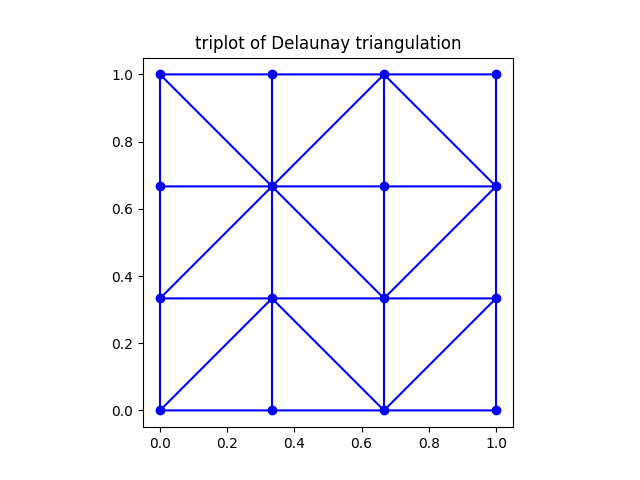
\includegraphics[scale = 0.6]{Figure_1.png}}
\end{figure} 


\subsection{Построение интерполянта}
Интерполянт задаётся в узлах сетки точными занчениями интерполируемой функции. На рёбрах конечного элемента он задаётся уравнением прямой в пространстве $R_3$, проходящей через точки ребра, на грани - уравнением плоскости, проходящей через вершины конечного элемента(в данной работе это впринципе не нужно, достаточно рассматривать рёбра).

\subsection{Вычисление нормы разности точного решения и интерполянта}

Норму считаем по следующей формуле
($\Omega_i$ - конечный элемент с индексом $i$, $N$ - число конечных элементов)
$$
||f||_{L_2(\Omega)} = \left(\int\limits_{\Omega}|f|^2d\Omega\right)^{0.5} = \left(\sum_{i=1}^{N}\int\limits_{\Omega_i}|f|^2d\Omega\right)^{0.5}
$$

А интеграл на конечном элементе считаем как:

$$
\int\limits_{\Omega_i}|f|^2d\Omega = \dfrac{\Delta_i}{3}(\psi_{12} + \psi_{13} + \psi_{23})
$$
Где $\psi_{jk}$ - значение функции $|f|^2$ в центральной точке ребра $jk$ конечного элемента $i$, \\
а $\Delta_i$ - площадь конечного элемента

При этом, в данном случае функция $f = u - u_I$. Пример того, как в точности вычисляется норма, есть в приведённом ниже коде программы

\subsection{Вычисление нормы разности градиентов точного решения и интерполянта}

Тут действуем в точности также, как и в пункте выше. В данном случае, функция $f = grad(u) - grad(u_I)$. $grad(u)$ задаём `вручную` по определению градиента. $grad(u_I)$ находим как сумму значений $a_1 + a_2$, где $a_1, a_2$ находим из решения системы:

\begin{equation}
 \begin{cases}
  a_1x_1 + a_2y_1 + a_3 = u(x_1, y_1) \\
  a_1x_2 + a_2y_2 + a_3 = u(x_2, y_2) \\
  a_1x_3 + a_2y_3 + a_3 = u(x_3, y_3)
 \end{cases}
 \nonumber
\end{equation}
Где $z = a_1x + a_2y + a_3$ - уравнение плоскости, в которой лежит конечный элемент, \\
а $(x_i, y_i, u(x_i, y_i))$ - координаты вершин конечного элемента (известны из постановки задачи и триангуляции области)

\subsection{Зависимость ошибки от числа шагов}

\begin{figure}[H] \label{fig1}
\centerline{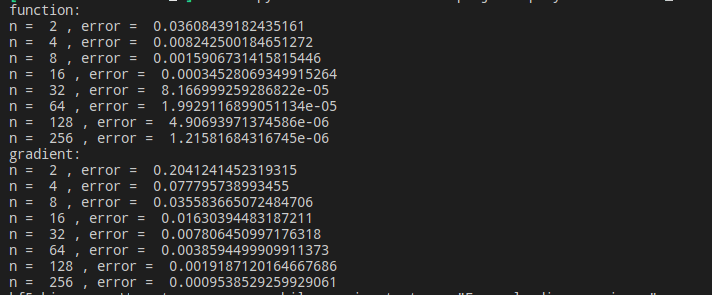
\includegraphics[scale = 0.6]{0.png}}
\end{figure} 

\begin{figure}[H] \label{fig1}
\centerline{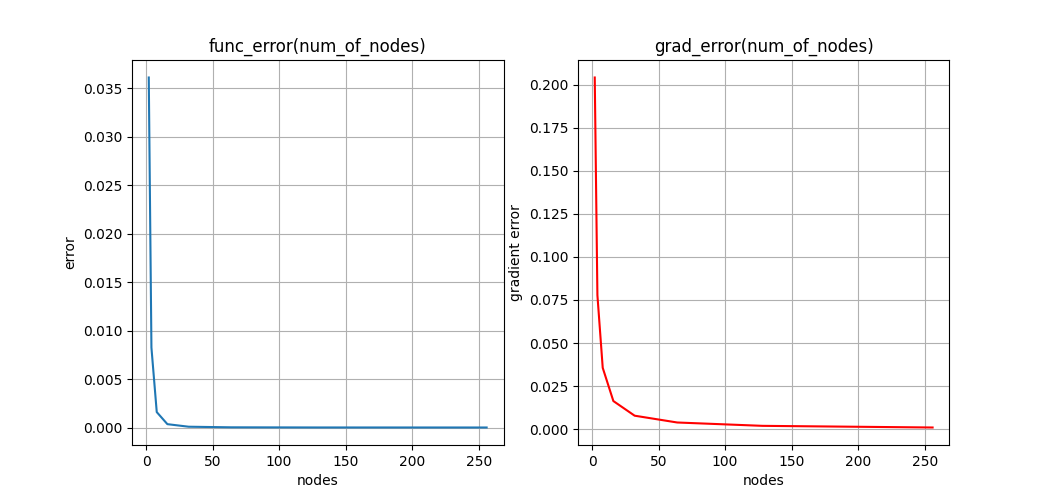
\includegraphics[scale = 0.6]{Figure_2.png}}
\end{figure} 

\section{Код}

Код программы можно посмотреть тут: \\
\url{https://github.com/LanskovNV/fem-labs/tree/master/lab_3}


\end{document}




























\end{document}
